\documentclass{standalone}
\usepackage{tikz}
\usetikzlibrary{patterns, positioning}
\usepackage[sfdefault]{ClearSans} %% option 'sfdefault' activates Clear Sans as the default text font
\usepackage[T1]{fontenc}

\begin{document}
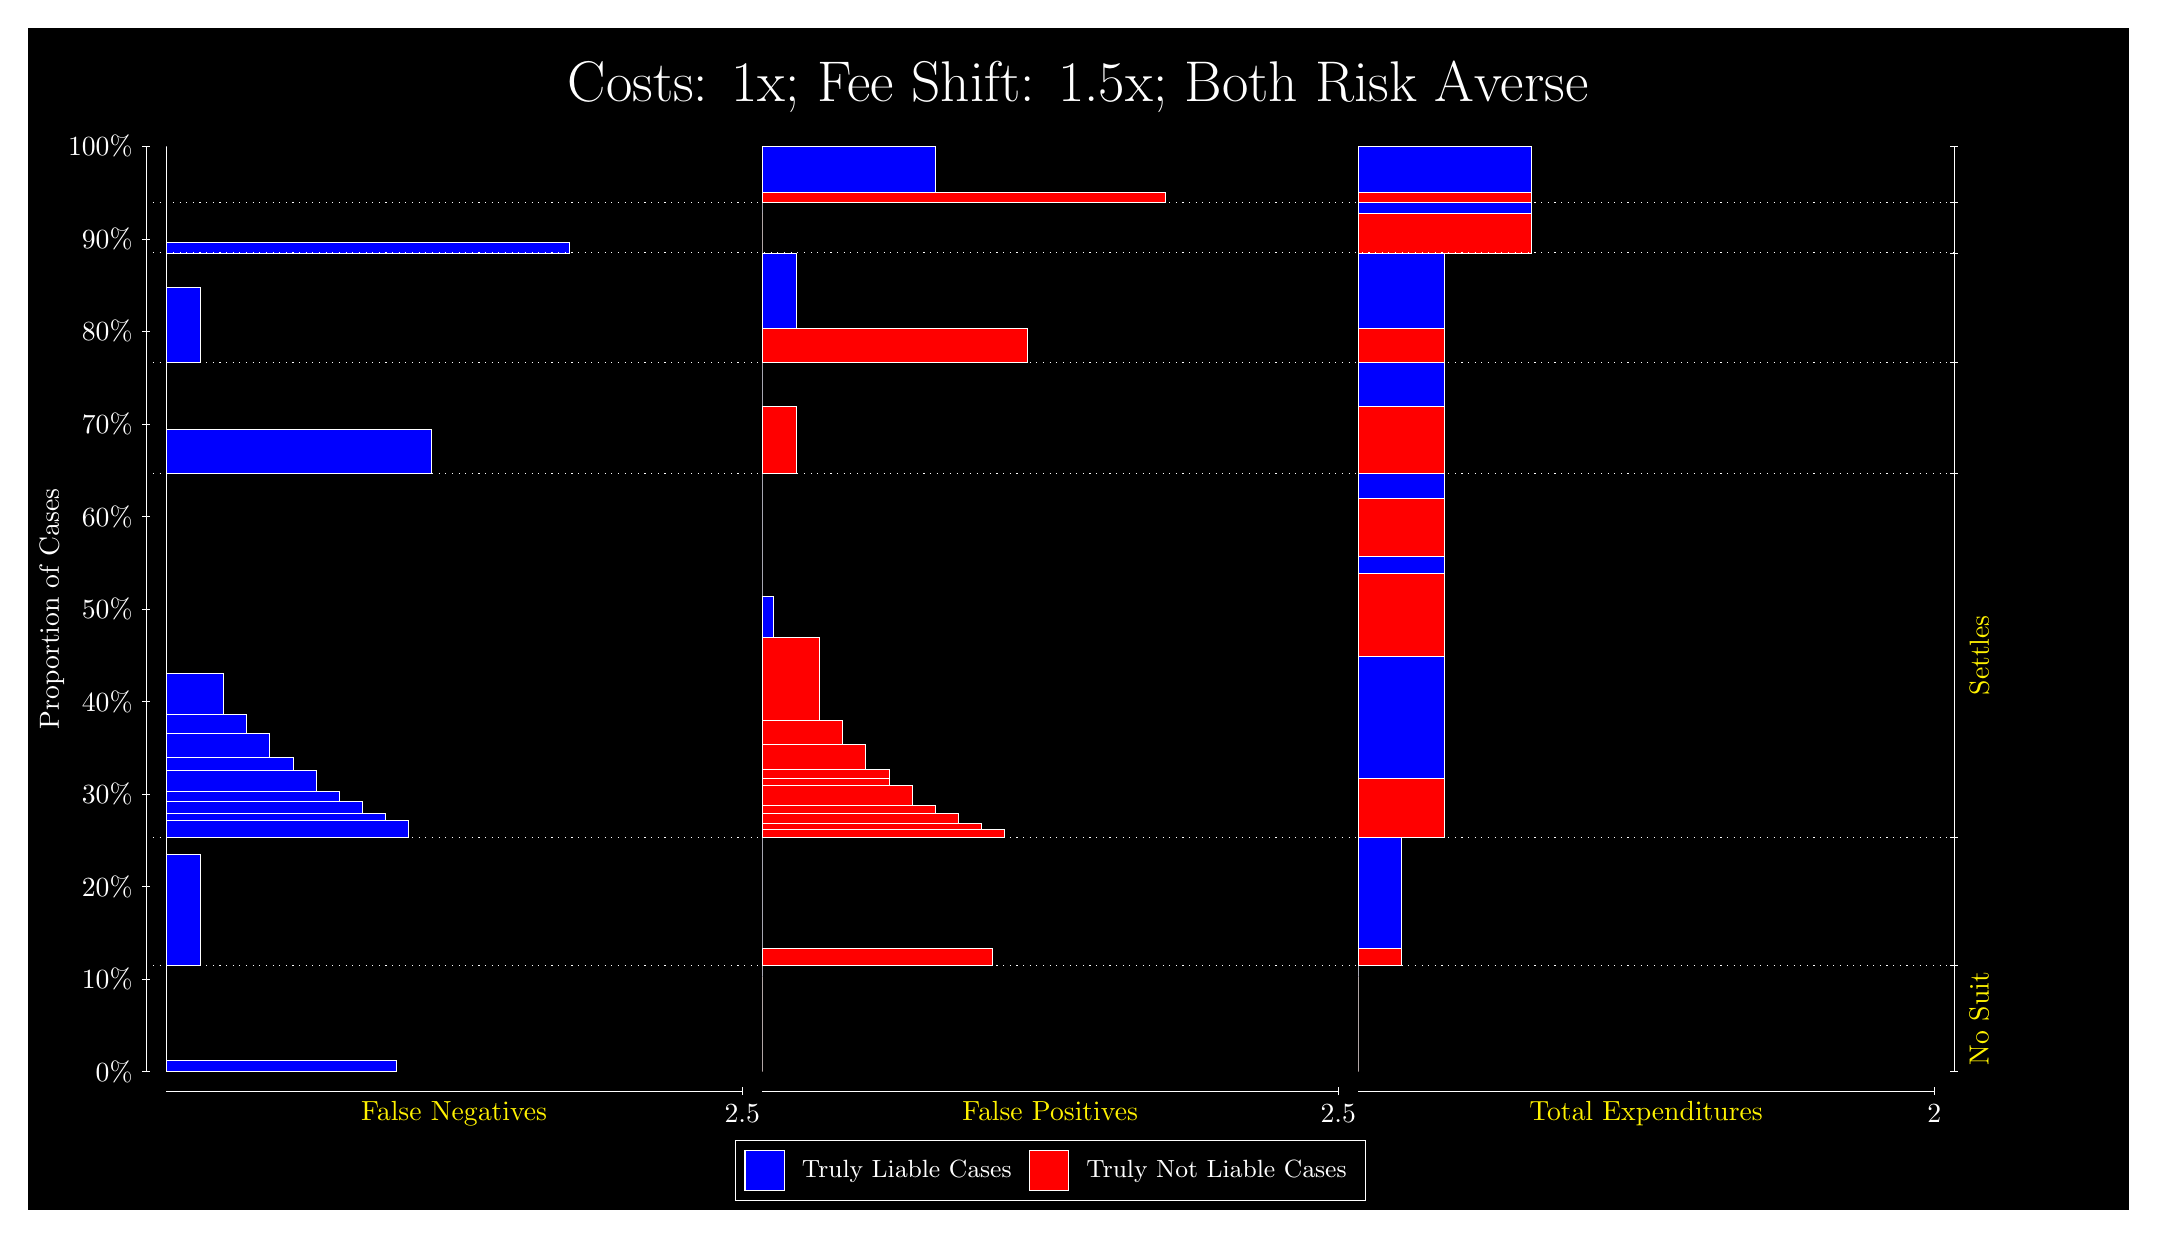
\begin{tikzpicture}
\draw[fill=black] (0,0) rectangle (26.667,15);
\draw[text=white] (0,13.5) rectangle (26.667,15) node[midway] {\huge Costs: 1x; Fee Shift: 1.5x; Both Risk Averse};
\draw[white, very thin] (1.5,1.75) -- (1.5,13.5);
\node[rotate=90, text=white, anchor=center] at (0.3, 7.625) {Proportion of Cases};
\draw[white, very thin] (1.45,1.75) -- (1.55,1.75);
\node[text=white, anchor=east] at (1.45, 1.75) {0\%};
\draw[white, very thin] (1.45,2.925) -- (1.55,2.925);
\node[text=white, anchor=east] at (1.45, 2.925) {10\%};
\draw[white, very thin] (1.45,4.1) -- (1.55,4.1);
\node[text=white, anchor=east] at (1.45, 4.1) {20\%};
\draw[white, very thin] (1.45,5.275) -- (1.55,5.275);
\node[text=white, anchor=east] at (1.45, 5.275) {30\%};
\draw[white, very thin] (1.45,6.45) -- (1.55,6.45);
\node[text=white, anchor=east] at (1.45, 6.45) {40\%};
\draw[white, very thin] (1.45,7.625) -- (1.55,7.625);
\node[text=white, anchor=east] at (1.45, 7.625) {50\%};
\draw[white, very thin] (1.45,8.8) -- (1.55,8.8);
\node[text=white, anchor=east] at (1.45, 8.8) {60\%};
\draw[white, very thin] (1.45,9.975) -- (1.55,9.975);
\node[text=white, anchor=east] at (1.45, 9.975) {70\%};
\draw[white, very thin] (1.45,11.15) -- (1.55,11.15);
\node[text=white, anchor=east] at (1.45, 11.15) {80\%};
\draw[white, very thin] (1.45,12.325) -- (1.55,12.325);
\node[text=white, anchor=east] at (1.45, 12.325) {90\%};
\draw[white, very thin] (1.45,13.5) -- (1.55,13.5);
\node[text=white, anchor=east] at (1.45, 13.5) {100\%};

\draw[white, very thin] (24.457,1.75) -- (24.457,13.5);
\draw[white, very thin] (24.407,1.75) -- (24.507,1.75);
\node[anchor=west] at (24.407, 1.75) {};
\draw[white, very thin] (24.407,3.0966) -- (24.507,3.0966);
\node[anchor=west] at (24.407, 3.0966) {};
\draw[white, very thin] (24.407,4.7268) -- (24.507,4.7268);
\node[anchor=west] at (24.407, 4.7268) {};
\draw[white, very thin] (24.407,9.3458) -- (24.507,9.3458);
\node[anchor=west] at (24.407, 9.3458) {};
\draw[white, very thin] (24.407,10.756) -- (24.507,10.756);
\node[anchor=west] at (24.407, 10.756) {};
\draw[white, very thin] (24.407,12.147) -- (24.507,12.147);
\node[anchor=west] at (24.407, 12.147) {};
\draw[white, very thin] (24.407,12.787) -- (24.507,12.787);
\node[anchor=west] at (24.407, 12.787) {};
\draw[white, very thin] (24.407,13.5) -- (24.507,13.5);
\node[anchor=west] at (24.407, 13.5) {};

\draw[white, very thin, fill=blue] (1.75,1.75) rectangle (4.6775,1.8917);
\draw[white, very thin, fill=red] (1.75,1.8917) rectangle (1.75,3.0966);
\draw[white, very thin, fill=blue] (1.75,3.0966) rectangle (2.1891,4.5094);
\draw[white, very thin, fill=red] (1.75,4.5094) rectangle (1.75,4.7268);
\draw[white, very thin, fill=blue] (1.75,4.7268) rectangle (4.8239,4.9434);
\draw[white, very thin, fill=blue] (1.75,4.9434) rectangle (4.5312,5.034);
\draw[white, very thin, fill=blue] (1.75,5.034) rectangle (4.2384,5.1832);
\draw[white, very thin, fill=blue] (1.75,5.1832) rectangle (3.9457,5.3135);
\draw[white, very thin, fill=blue] (1.75,5.3135) rectangle (3.6529,5.5723);
\draw[white, very thin, fill=blue] (1.75,5.5723) rectangle (3.3602,5.7357);
\draw[white, very thin, fill=blue] (1.75,5.7357) rectangle (3.0674,6.0493);
\draw[white, very thin, fill=blue] (1.75,6.0493) rectangle (2.7746,6.2882);
\draw[white, very thin, fill=blue] (1.75,6.2882) rectangle (2.4819,6.8132);
\draw[white, very thin, fill=red] (1.75,6.8132) rectangle (1.75,9.3458);
\draw[white, very thin, fill=blue] (1.75,9.3458) rectangle (5.1167,9.9094);
\draw[white, very thin, fill=red] (1.75,9.9094) rectangle (1.75,10.756);
\draw[white, very thin, fill=blue] (1.75,10.756) rectangle (2.1891,11.715);
\draw[white, very thin, fill=red] (1.75,11.715) rectangle (1.75,12.147);
\draw[white, very thin, fill=blue] (1.75,12.147) rectangle (6.8732,12.282);
\draw[white, very thin, fill=red] (1.75,12.282) rectangle (1.75,12.787);
\draw[white, very thin, fill=red] (1.75,12.787) rectangle (1.75,12.922);
\draw[white, very thin, fill=blue] (1.75,12.922) rectangle (1.75,13.5);
\draw[white, very thin, fill=red] (9.3189,1.75) rectangle (9.3189,2.9549);
\draw[white, very thin, fill=blue] (9.3189,2.9549) rectangle (9.3189,3.0966);
\draw[white, very thin, fill=red] (9.3189,3.0966) rectangle (12.246,3.314);
\draw[white, very thin, fill=blue] (9.3189,3.314) rectangle (9.3189,4.7268);
\draw[white, very thin, fill=red] (9.3189,4.7268) rectangle (12.393,4.8208);
\draw[white, very thin, fill=red] (9.3189,4.8208) rectangle (12.1,4.8976);
\draw[white, very thin, fill=red] (9.3189,4.8976) rectangle (11.807,5.025);
\draw[white, very thin, fill=red] (9.3189,5.025) rectangle (11.515,5.1288);
\draw[white, very thin, fill=red] (9.3189,5.1288) rectangle (11.222,5.3888);
\draw[white, very thin, fill=red] (9.3189,5.3888) rectangle (10.929,5.472);
\draw[white, very thin, fill=red] (9.3189,5.472) rectangle (10.929,5.5831);
\draw[white, very thin, fill=red] (9.3189,5.5831) rectangle (10.636,5.9121);
\draw[white, very thin, fill=red] (9.3189,5.9121) rectangle (10.344,6.212);
\draw[white, very thin, fill=red] (9.3189,6.212) rectangle (10.051,7.2594);
\draw[white, very thin, fill=blue] (9.3189,7.2594) rectangle (9.4652,7.7844);
\draw[white, very thin, fill=blue] (9.3189,7.7844) rectangle (9.3189,9.3458);
\draw[white, very thin, fill=red] (9.3189,9.3458) rectangle (9.758,10.193);
\draw[white, very thin, fill=blue] (9.3189,10.193) rectangle (9.3189,10.756);
\draw[white, very thin, fill=red] (9.3189,10.756) rectangle (12.686,11.189);
\draw[white, very thin, fill=blue] (9.3189,11.189) rectangle (9.758,12.147);
\draw[white, very thin, fill=red] (9.3189,12.147) rectangle (9.3189,12.652);
\draw[white, very thin, fill=blue] (9.3189,12.652) rectangle (9.3189,12.787);
\draw[white, very thin, fill=red] (9.3189,12.787) rectangle (14.442,12.922);
\draw[white, very thin, fill=blue] (9.3189,12.922) rectangle (11.515,13.5);
\draw[white, very thin, fill=red] (16.888,1.75) rectangle (16.888,2.9549);
\draw[white, very thin, fill=blue] (16.888,2.9549) rectangle (16.888,3.0966);
\draw[white, very thin, fill=red] (16.888,3.0966) rectangle (17.437,3.314);
\draw[white, very thin, fill=blue] (16.888,3.314) rectangle (17.437,4.7268);
\draw[white, very thin, fill=red] (16.888,4.7268) rectangle (17.986,5.472);
\draw[white, very thin, fill=blue] (16.888,5.472) rectangle (17.986,7.0263);
\draw[white, very thin, fill=red] (16.888,7.0263) rectangle (17.986,8.0737);
\draw[white, very thin, fill=blue] (16.888,8.0737) rectangle (17.986,8.2903);
\draw[white, very thin, fill=red] (16.888,8.2903) rectangle (17.986,9.0303);
\draw[white, very thin, fill=blue] (16.888,9.0303) rectangle (17.986,9.3458);
\draw[white, very thin, fill=red] (16.888,9.3458) rectangle (17.986,10.193);
\draw[white, very thin, fill=blue] (16.888,10.193) rectangle (17.986,10.756);
\draw[white, very thin, fill=red] (16.888,10.756) rectangle (17.986,11.189);
\draw[white, very thin, fill=blue] (16.888,11.189) rectangle (17.986,12.147);
\draw[white, very thin, fill=red] (16.888,12.147) rectangle (19.083,12.652);
\draw[white, very thin, fill=blue] (16.888,12.652) rectangle (19.083,12.787);
\draw[white, very thin, fill=red] (16.888,12.787) rectangle (19.083,12.922);
\draw[white, very thin, fill=blue] (16.888,12.922) rectangle (19.083,13.5);
\draw[white, dotted] (1.5,3.0966) -- (24.457,3.0966);
\draw[white, dotted] (1.5,4.7268) -- (24.457,4.7268);
\draw[white, dotted] (1.5,9.3458) -- (24.457,9.3458);
\draw[white, dotted] (1.5,10.756) -- (24.457,10.756);
\draw[white, dotted] (1.5,12.147) -- (24.457,12.147);
\draw[white, dotted] (1.5,12.787) -- (24.457,12.787);
\draw[white, very thin] (1.75,1.5) -- (9.0689,1.5);
\node[text=yellow, anchor=north] at (5.4094, 1.5) {False Negatives};
\draw[white, very thin] (9.0689,1.45) -- (9.0689,1.55);
\node[text=white, anchor=north] at (9.0689, 1.45) {2.5};

\draw[white, very thin] (9.3189,1.5) -- (16.638,1.5);
\node[text=yellow, anchor=north] at (12.978, 1.5) {False Positives};
\draw[white, very thin] (16.638,1.45) -- (16.638,1.55);
\node[text=white, anchor=north] at (16.638, 1.45) {2.5};

\draw[white, very thin] (16.888,1.5) -- (24.207,1.5);
\node[text=yellow, anchor=north] at (20.547, 1.5) {Total Expenditures};
\draw[white, very thin] (24.207,1.45) -- (24.207,1.55);
\node[text=white, anchor=north] at (24.207, 1.45) {2};

\node[text=yellow, centered, rotate=90] at (24.777, 2.4233) {No Suit};

\node[text=yellow, centered, rotate=90] at (24.777, 7.0363) {Settles};





\draw (12.978300999999998,1.5) node[draw=none] (baseCoordinate) {};
\begin{scope}[align=center]
        \matrix[scale=0.5, draw=white, below=0.5cm of baseCoordinate, nodes={draw}, column sep=0.1cm]{
            \node[rectangle, draw, minimum width=0.5cm, minimum height=0.5cm, fill=blue] {}; &
            \node[draw=none, font=\small, text=white] (B) {Truly Liable Cases}; &
            \node[rectangle, draw, minimum width=0.5cm, minimum height=0.5cm, fill=red] {}; &
            \node[draw=none, font=\small, text=white] (B) {Truly Not Liable Cases}; \\
            };
\end{scope}

\end{tikzpicture}
\end{document}